% This text is proprietary.
% It's a part of presentation made by myself.
% It may not used commercial.
% The noncommercial use such as private and study is free
% Sep. 2005 
% Author: Sascha Frank 
% University Freiburg 
% www.informatik.uni-freiburg.de/~frank/


\documentclass{beamer}
\usecolortheme{whale}
\useoutertheme{split}
\usefonttheme[onlysmall]{structurebold}
\begin{document}
%\title{Simple Beamer Class}   
%\author{Sascha Frank} 
%\date{\today} 

%\frame{\titlepage} 

\frame{\frametitle{Table of contents}\tableofcontents} 

\section{Problem Statement}

\frame{

\frametitle{Does a 6 bit counter exists ?} 

Can we create a \textbf{deterministic} network that will iterate over all 6 bits string -- in any order -- ?

}

\frame{
\frametitle{Does a 6 bit counter exists ?} 
\center{
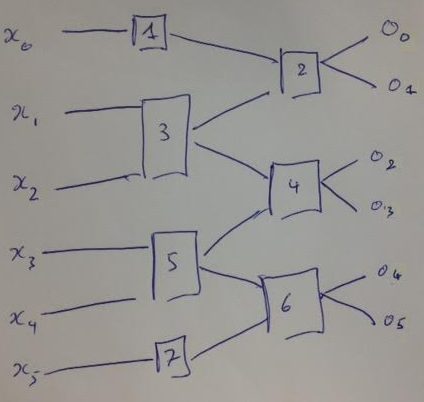
\includegraphics[scale=0.7]{netk.png}
}

}


\frame{\frametitle{Can we bruteforce that problem ?}
There are $\boldsymbol{2^{44}}$ differents networks which is approximatively $17 000$ billions.\\
We could hope for an answer in a few days.\\
\textbf{But} we can drastically restrict our search space with a \textbf{few} observations.\\ \ \\

\textbf{Main idea :} we are going to bruteforce on \textbf{sub networks} and select those who respect a \textbf{necessary} condition.
} 


\frame{\frametitle{How such a network's dynamic would look like ?} 

There are only two possibilities (up to any permutation):
\rotatebox{180}{
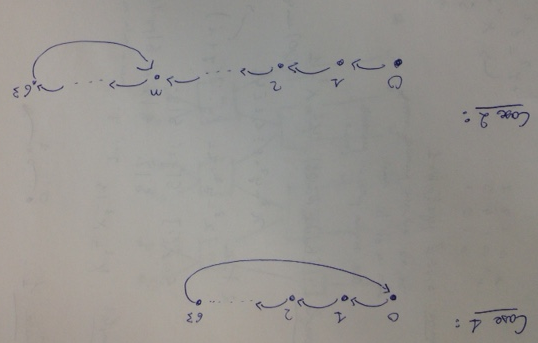
\includegraphics[scale=0.7]{2cases.png}
}


}

\frame{\frametitle{Implication on the computed function  by the network} 

The function that our counting network coumputes is either:
\begin{itemize}
\item \textbf{A bijection}
\item \textbf{An almost-bijection} $f$ i.e, $\exists ! x_0,y_0 \in \{0,1\}^6$ such that $f'$ is a bijection where:  
\begin{align*}
\forall x \neq x_0 \quad & f'(x) = f(x) \\
& f'(x_0) = y_0 \\
\end{align*}
We are going to check on both cases.
\end{itemize} 
}

\section{Computable bijections on $\{0,1\}^6$}
\subsection{4*16 property}
\frame{\frametitle{The $4*16$ property} 

If we have a bijection it will \textbf{enumerate} all strings of  
$\{0,1\}^6$. After reordordering it will look like:\\ \ \\
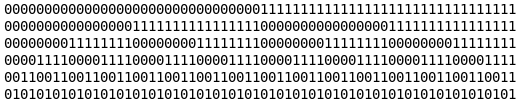
\includegraphics[scale=0.6]{all6b.png}

}

\frame{\frametitle{The $4*16$ property} 

Let's focus on the first two bits, we can organise our sequences this way: \\ \ \\
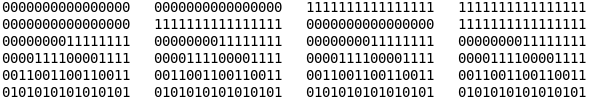
\includegraphics[scale=0.55]{all6b2b.png}
}
\frame{\frametitle{The $4*16$ property} 

Let get rid of the last 4 bits: \\ \ \\

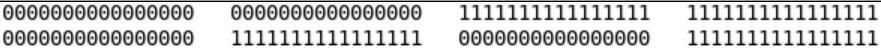
\includegraphics[scale=0.45]{6b2b.png}

\ \\ 

We see that each of the 2 bits patterns:  \textbf{00, 01, 10, 11} occurs \textbf{16} times in this enumeration.\\
It's the \textbf{$\boldsymbol{4*16}$ property}.

}

\frame{\frametitle{The $4*16$ property} 

\textbf{Hence} the sub network responsible for these 2 bits must have the \textbf{4*16} property to be eligible as a being a sub network of a 6 bits bijective counter network.

}

\frame{\frametitle{The $4*16$ property} 

\rotatebox{90}{
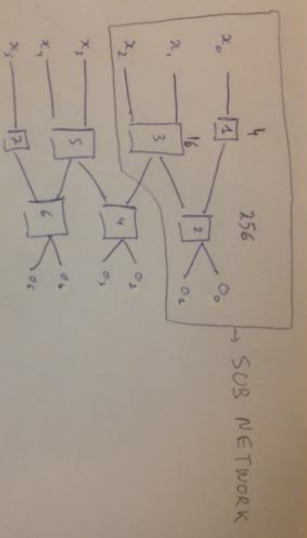
\includegraphics[scale=0.8]{subnetk.png}
}


}

\frame{\frametitle{Compute all the $4*16$ sub networks} 

By exausthive search we find $\boldsymbol{288}$ (over $4*16*256=16384$) sub networks with this property. \\ \ \\

By removing equivalent networks we are left with \textbf{$\boldsymbol{72}$ circuits for the first 2 bits}.

}

\subsection{Combine}

\frame{\frametitle{4*16 holds for middle and ending bits}

\rotatebox{90}{
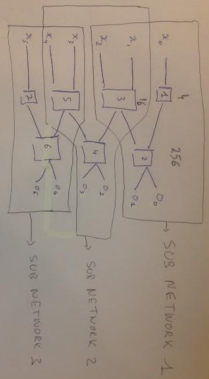
\includegraphics[scale=1.1]{subnetsk.png}
}


}

\frame{\frametitle{4*16 holds for middle and ending bits}

\begin{itemize}
\item \textbf{72} networks for the first 2 bits
\item \textbf{216} networks for the middle 2 bits
\item \textbf{72} networks for the last 2 bits
\end{itemize}

}

\subsection{Conclude}

\frame{\frametitle{How to conclude I ? Combine it !}


\textbf{Hence} by combining these we have $72*216*72 \simeq 10^6$ \\ 6 bits networks to test.

} 

\frame{\frametitle{How to conclude II ? Count orbits !}

Over all these potential networks we count $\boldsymbol{497664}$ bijections. \\
For each of these bijections we have to \textbf{count their orbits}, we have a winner \textbf{iif it has only 1 orbit}. \\ \ \\
We do not find such a network, here there's the histogram of orbits: \\

\center

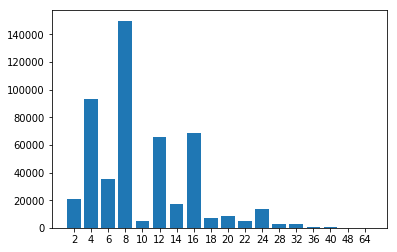
\includegraphics[scale=0.46]{hist_orbits.png}

} 

\frame{\frametitle{Conclusion}
\textbf{Conclusion:} There are no bijective 6bits counters.
}


\section{Computable almost-bijections on $\{0,1\}^6$}
\subsection{2*161517 property}

\frame{\frametitle{2*161517 property}

If we have an almost-bijection \textbf{all 6 bits sequences will be reached by our network but one}.\\ \ \\
Also one bit string will be reached \textbf{twice}. \\ \ \\
It means that \textbf{at least one} of our sub network will see:
\begin{itemize}
\item 2 patterns \textbf{16} times
\item 1 pattern \textbf{15} times
\item 1 pattern \textbf{17} times
\end{itemize}
}

\frame{\frametitle{2*161517 property}

We call this the \textbf{2*161517 property}.

}
\subsection{Conclusion}
\frame{\frametitle{2*161517 does not occur !}

By enumeration, \textbf{there exist no sub network with the 2*161517} property. \\
\textbf{Hence}, we cannot hope for an \textbf{almost-bijective counter}.

}

\section{Conclusion}
\frame{\frametitle{No 6bit counter network :'( }

By case distinction, \textbf{there's no 6bit counter network}.
\\ \
But there are \textbf{0 to 62} counters and this kind of methods helps to exhibit \textbf{at least 24}.
}

\frame{\frametitle{Sources ? }

All our sources for these computations are available here: \\ \ \\
\url{https://github.com/cosmo-sterin/ER_MolProg_Project2/tree/master/circuit_sim}
}

\end{document}
